\section{Results and Analysis}\label{sec:simulations}
The specified specifications are verified by the use of simulations. While providing a one tone signal, a transient measurement of the output power is simulated. This to verify a correct functioning DAC, that translates the digitals signals as supposed. This holds that the 15 bit digital unary code is translated to an analogue signal.
\begin{figure}[htp] 
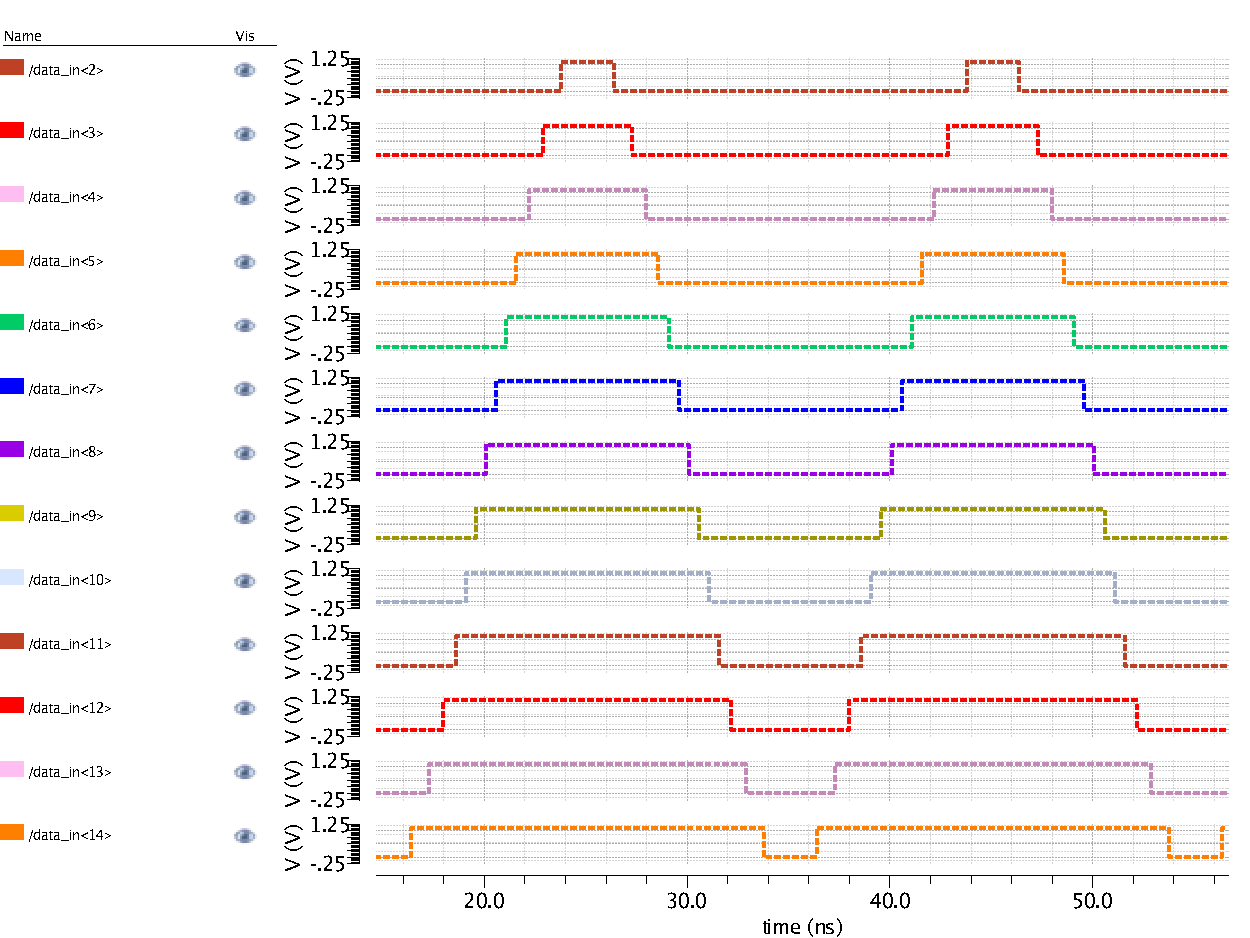
\includegraphics[width=0.5\textwidth]{thermometer_output.pdf}
\caption{Thermometer single tone voltage output.}
\label{fig:Thermometer}
\end{figure}
\begin{figure}[htp] 
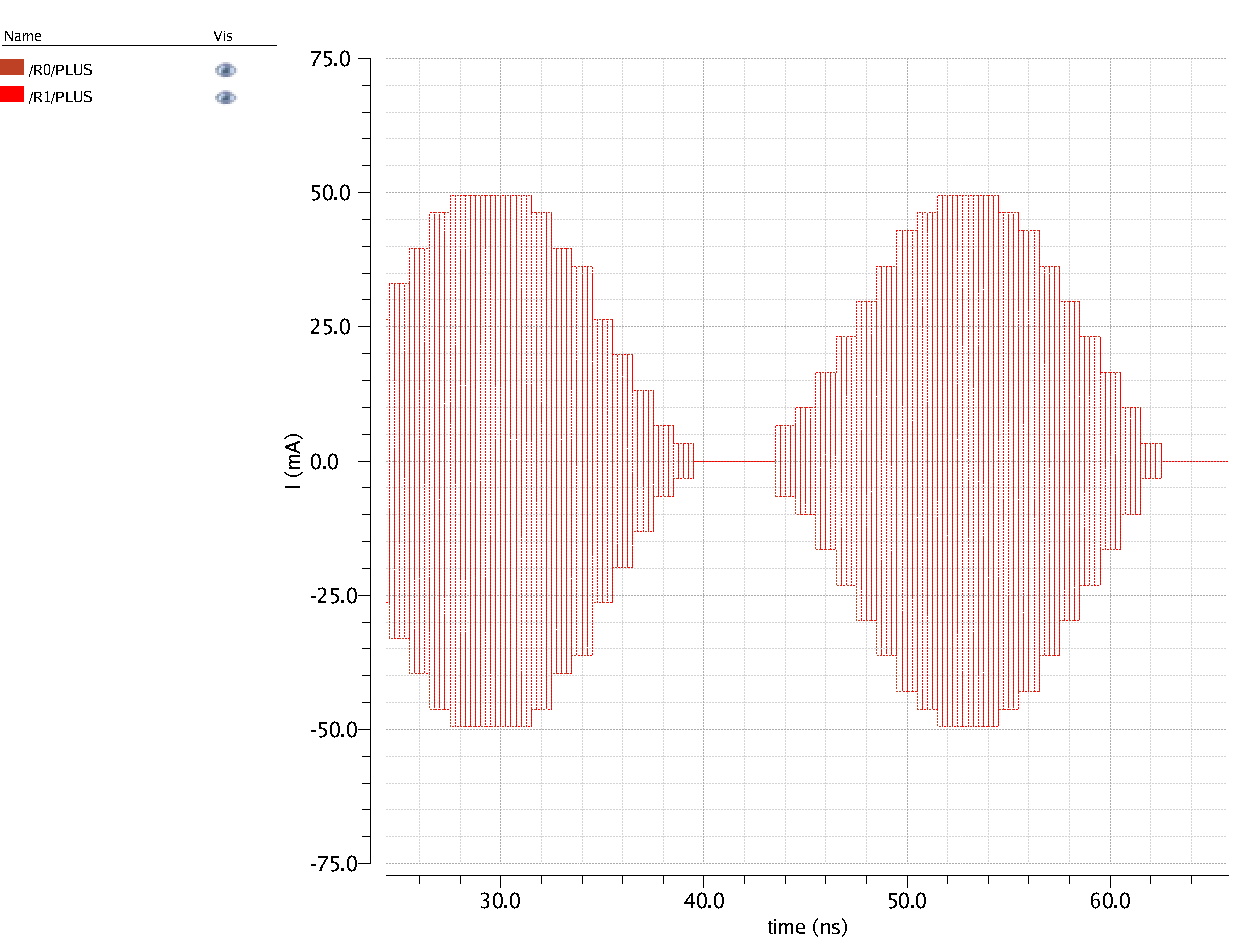
\includegraphics[width=0.5\textwidth]{Iout_ideal.pdf}
\caption{Output current}
\label{fig:Output current}
\end{figure}
Next a DFT of the output voltage is simulated to see the spectral content of the one tone model. To simulate such a DFT the simulation duration should be chosen wisely, an integer number multiple of the period time, otherwise a single tone will not be shown as a single point in the spectrum. The simulation time is chosen to be 512 LO periods and the first 10 periods are neglected to filter out settling issues. To fit exactly 11 IF periods in this timespan the IF frequency should be 42.97 MHz.
\begin{figure}[htp] 
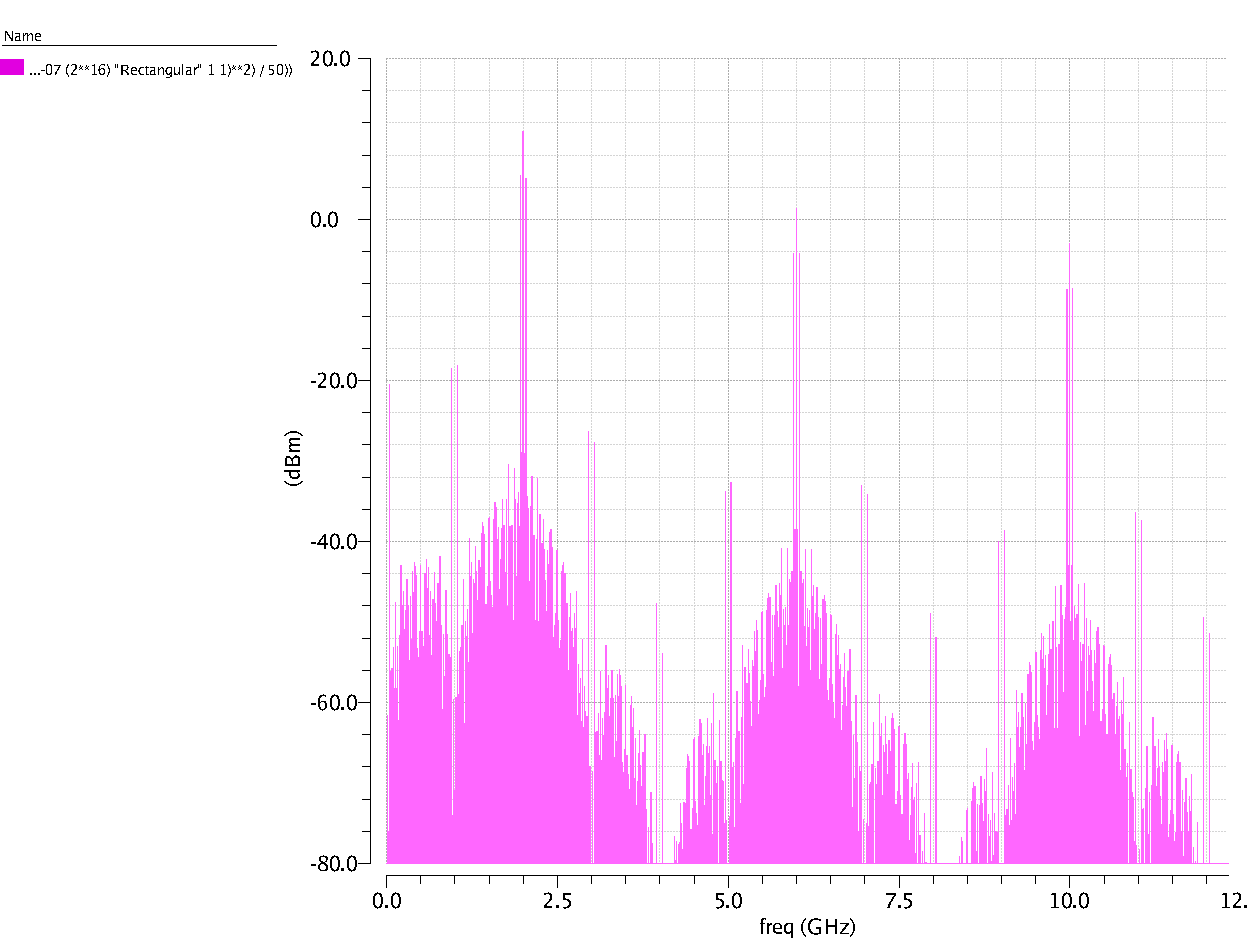
\includegraphics[width=0.5\textwidth]{DFT_one_tone.pdf}
\caption{Single tone spectrical content}
\label{fig:Single tone spectrical content}
\end{figure}
Furthermore a two tone test is simulated, the two tone test is useful test the linearity of the DAC. Non-linear behaviour generates intermodulation products at the output of the DAC. The power of these intermodulation products will examined, especially the third intermodulation product (IM3). Because the IM3 frequencies are very close to the fundamental frequency (at 2f2-f1 and 2f1-f2), it is almost impossible to filter it out of the output signal; therefore, it is better to prevent creating them.
\begin{figure}[htp] 
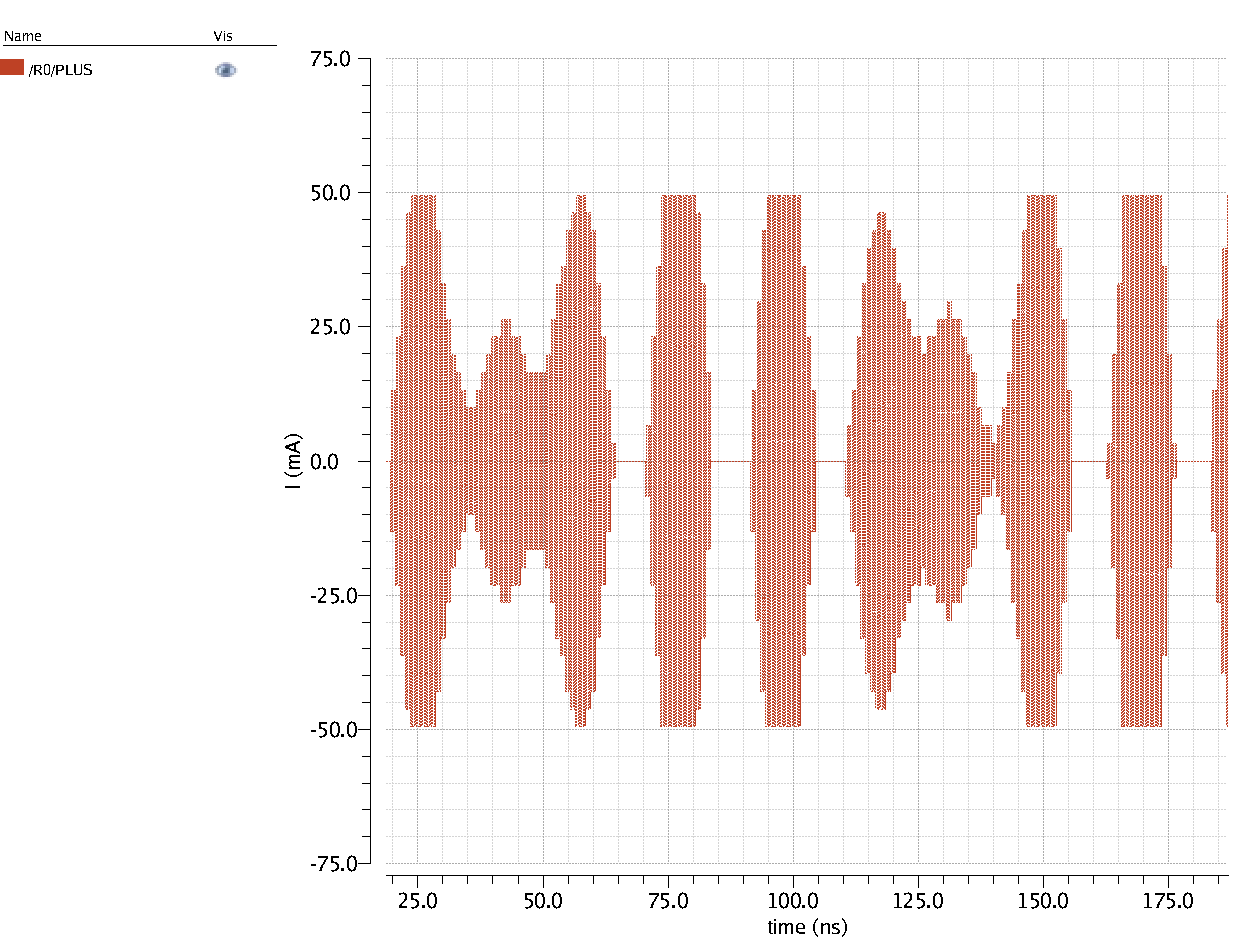
\includegraphics[width=0.5\textwidth]{trans_two_tone.pdf}
\caption{Two tone output current}
\label{Two tone output current}
\end{figure}
The spectral image of this two tone test is useful to find the power of the total harmonic distortion (THD) and the spurious-free dynamic range (SFDR).  The SFDR describes the power of the fundamental signal to the strongest spurious signal at the output, which is in this case the IM3. The frequency of the second tone is chosen so that 14 cycles fit in the simulation time, which means that the IF frequency of the second tone is equal to 54.69 MHz.
